\section{Miami Grand prix}

\subsection{Circuit Analysis}

\textbf{Circuit Name:} Miami International Autodrome (Miami, USA) \\
\textbf{Length:} 5.412 km - \textbf{Laps:} 57 - \textbf{Total Distance:} 308.326 km

\begin{figure}[H]
    \centering
    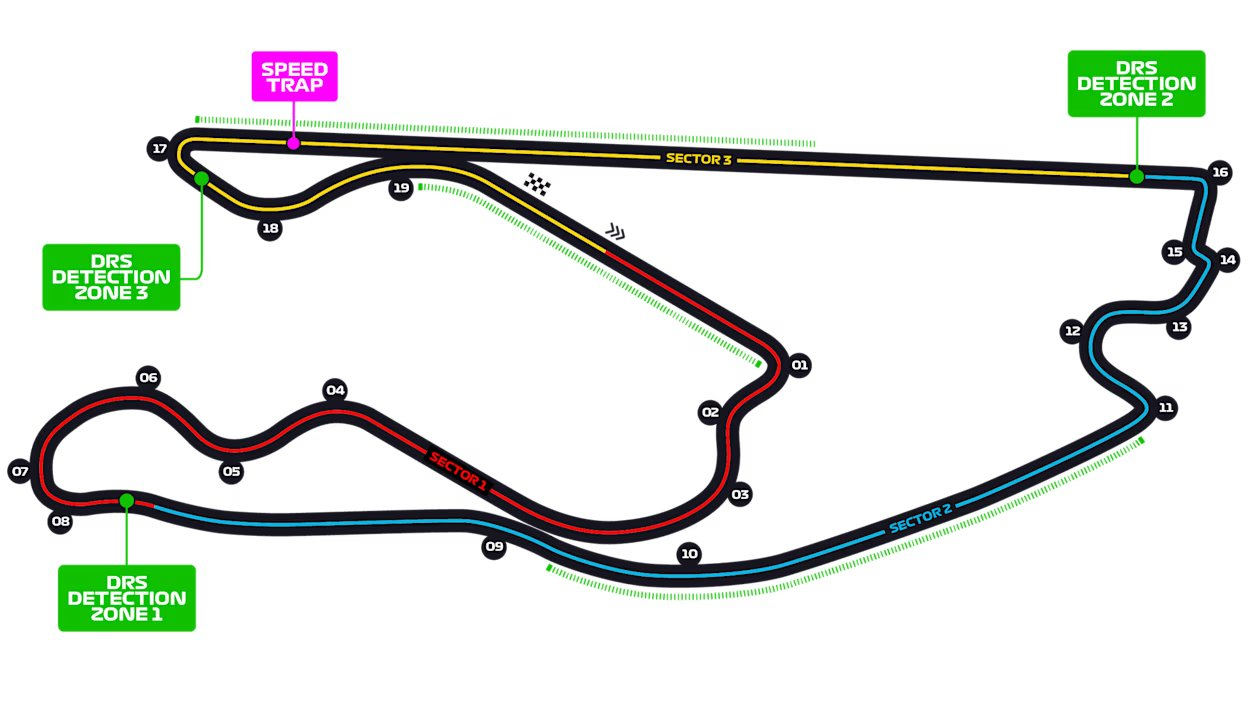
\includegraphics[width=0.75\linewidth]{images/6.Miami_Circuit.jpg}
\end{figure}

\begin{itemize}
    \item \textbf{Lap Record} : 1:26.841 (2023, Sergio Pérez - Red Bull).
    
    \item \textbf{Number of Corners \& Key Features} : 19 turns (7 right, 12 left) - Combination of fast sections (Turns 4–8), long back straight into heavy braking at Turn 17, and a tight, technical complex between Turns 11–16.
    
    \item \textbf{Braking Zones \& Traction} : Heavy braking at Turn 17 (from ~320 km/h down to 70 km/h). Traction crucial out of Turn 16 leading onto the long straight.
    
    \item \textbf{DRS \& Overtaking} : Three DRS zones (between Turns 9–11, 16–17, and main straight). Best overtaking chances at Turn 11 and Turn 17.
    
    \item \textbf{Tyre Degradation \& Strategy} : Tyre wear relatively low but thermal degradation high due to heat. \\
    One-stop strategies favoured, though Safety Cars can shuffle plans.
    
    \item \textbf{Weather \& Environment} : Hot and humid conditions typical of Miami in May.\\
    Track surface is new and evolving, often slippery off-line.\\
    Risk of thunderstorms and high humidity affects grip and cooling.
\end{itemize}

\textbf{Strategic Summary :}
Miami rewards cars with high straight-line speed and braking stability, while the technical sector demands strong low-speed traction. Tyre management and cooling are critical due to high ambient temperatures. Safety Cars are common and can be decisive.


\subsection{Race Analysis}

\textbf{Date:} Sprint : 4 May 2024 - 12:00 local time\\
Race : 5 May 2024 — 16:00 local time 

\begin{itemize}
    \item \textbf{Sprint Qualifying:} \textbf{Pole Position:} Max Verstappen (Red Bull) - 1:27.641.\\
    Grid : Leclerc 2nd, Pérez 3rd, Ricciardo 4th.

    \item \textbf{Sprint Summary} : \textbf{Winner:} Max Verstappen (Red Bull). \\
    \textbf{Podium}: 1. Verstappen - 2. Leclerc - 3. Pérez. \\
    Hamilton triggered contact at Turn 1 (+ 20s) → Alonso + Stroll caught out, Norris spun and retired.\\
    Ricciardo finished P4, Tsunoda scored P8. 
    
    \item \textbf{Qualifying Summary} : \textbf{Pole Position:} Max Verstappen (Red Bull) – 1:27.241. \\
    Grid: Leclerc 2nd, Sainz 3rd, Pérez 4th.
    
    \item \textbf{Race Summary} : \textbf{Winner:} Lando Norris (McLaren) - his first F1 victory\\
    \textbf{Podium:} 1. Norris - 2. Verstappen - 3. Leclerc.\\
    \textbf{Technical issues:} Hamilton (damage after early contact, retired lap 33).
    \textbf{Notable incidents:} Safety Car on lap 29 after Kevin Magnussen and Logan Sargeant collided, which allowed Norris to pit at the perfect time and undercut Verstappen.
    
    \item \textbf{Strategies} : Majority opted for one-stop.\\
    - Verstappen started on mediums then switched to hards (standard plan). \\
    - Norris benefited from pitting under the Safety Car (Medium–Hard with track position gain).\\
    - Ferrari followed conservative Medium–Hard but lacked late pace.
    
    \item \textbf{Performance Trends} : \textbf{McLaren} — Major upgrades transformed pace. Norris flawless, Piastri unlucky with contact.\\
    \textbf{Red Bull} — Verstappen still dominant in pace, but strategy luck beat him. Pérez only P4.\\
    \textbf{Ferrari} — Strong consistency: Leclerc on podium, Sainz P5.\\
    \textbf{Mercedes} — Decent recovery, solid points but off the front-running pace.\\
    \textbf{Midfield} — Tsunoda shined P7. Alonso salvaged P9 despite weak weekend. Ocon scored Alpine’s first point of 2024.
    
    \item \textbf{Championship Impact} : \textbf{Drivers:} Verstappen 136 points, Pérez 103, Leclerc 98.\\
    \textbf{Constructors:} Red Bull 239, Ferrari 187, McLaren 124, Mercedes 64.    
\end{itemize}

\textbf{Key Takeaway :}
Norris and McLaren seized their moment, perfectly exploiting the Safety Car. Red Bull remained the benchmark in raw pace, but Miami proved strategy and timing can beat outright speed.


\subsection{Link \& Takeaway}

\begin{itemize}
    \item Miami’s long straights and heavy braking zones usually favour Red Bull, but the Safety Car timing flipped the race. 
    \item Ferrari showed consistency but lacked outright pace to fight for the win.
    \item Miami’s Safety Car timing completely reshuffled the order, benefiting Norris. 
    \item McLaren’s upgrades paid off instantly, transforming potential into a breakthrough win. 
    \item Alpine finally scored points. Tsunoda and Racing Bulls continued strong midfield form.
\end{itemize}